%=========================================================================
% (c) Petr Stehlík, 2016

%\usepackage{xcolor}
\newcommand\note[1]{{\Large \textcolor{red}{#1}}}

\chapter{Úvod}
Počítačové sítě, zejména Internet, v dnešním světě zaujímají jednu z nejvýznamnějších rolí. Počínaje výzkumem a vědeckými experimenty, konče běžným životem většiny lidí. Jen za posledních deset let se počet uživatelů Internetu více než ztrojnásobil z přibližně jedné miliardy na tři miliardy uživatelů. Počítačové sítě propujují celý svět a jsou neustále rozšiřovány, vylepšovány a modernizovány. To vede k větším nárokům na použité technologie a zdroje. 

Avšak se zvyšujícím počtem uživatelů roste i počet útoků na různé počítačové sítě, kterými se útočníci snaží získat informace či poškodit oběť. Síťový útok je podle \cite{rfc:attack} definován jako záměrný akt, kde se entita snaží překonat bezpečnostní služby a porušit bezpečnost systému. Současně s tím vznikají systémy na detekci takovýchto útoků, aby správcí sítí dokázali včas a efektivně reagovat na vzniklou situaci.

Jeden z těchto systémů vznikl ve sdružení CESNET s názvem NEMEA (Network Measurements Analysis). Tento systém mj. slouží pro analýzu síťového provozu a detekci neobvyklých událostí na síti. Podezřelé toky jako agregované události pak může zaznamenávat  do databáze. Na větší síti (stovky až tisíce připojených zařízení) je takovýchto událostí vytvořeno až několik tisíc denně. S tím nastává problém jak dané události jednoduše analyzovat a rozpoznat na jaké události se zaměřit a na které nebrát zřetel.

Pro efektivní analýzu velkého množství dat je vhodná vizualizace dle vhodných metrik, které vyplývají z dostupných dat. Cílem této bakalářské práce je vytvořit aplikaci pro vizuální analýzu bezpečnostních událostí na síti primárně monitorované systémem NEMEA, nicméně díky IDEA formátu dat bude aplikace přenositelná na další systémy. 

Důležitým aspektem vytvořené aplikace je důraz na použití moderních knihoven podporující tvorbu dynamických webových aplikací, které jsou dostupné na různých typech zařízeních. Společně s tím je kladen důraz na uživatelskou přívětivost a jednoduchost prostředí, ve kterém bude probíhat vizuální analýza událostí.

Celou aplikaci navíc bude možno libovolně přizpůsobit tak, aby vyhovovala potřebám daného správce sítě. V aplikaci bude zavedena technika {\it drill-down}, která napomáhá rychlé a přehledné analýze velkého množství dat bez ztráty informací o analyzované události. Drill-down spočívá v postupném zvyšování rozlišení dat, která analyzujeme a postupujeme směřem shora dolů.

Aplikace bude pracovat s konkrétním formátem dat nazvaný IDEA. Tento formát dat je specifikován sdružením CESNET a slouží jako prostředek pro sdílení dat bezpečnostních událostí mezi různými systémy. Díky tomu lze systém kdykoliv přenést na jiný zdroj databáze než je systém NEMEA, např. v rámci sdružení CESNET na systém Warden nebo Mentat.

Aplikace bude integrována do současného NEMEA systému pod názvem NEMEA Dashboard a bude s ním společně distribuována jako front~end celého systému.

\chapter{Monitorování sítě}

V rozlehlejších sítích jako je např. páteřní či firemní síť je téměř nutností monitorovat a analyzovat provoz na síti, abychom byli informování o jejím aktuálním stavu, vytížení a zejména negativních vlivech na monitorovanou síť. Samozřejmě i sítě menšího rozsahu by měly být monitorované. Pokud se v malé firmě podaří útočníkovi infiltrovat síť, výsledky útoku mohou být pro firmu likvidační.

Systém pro odhalení průniku (anglicky \uv{Intrusion Detection System}, zkráceně IDS)\cite{idsips} je takový systém, který analyzuje a identifikuje ze zachyceného provozu podezřelé události. Tyto události může IDS dále klasifikovat. IDS může být dvojího typu. 

Prvním typem je detekce anomálií, který má výhodu v možnosti detekce jak známých, tak neznámých útoků. Nevýhodou je, že často může označit normální provoz za útok. Tomu se snaží předejít učením a tvorbou datové sady pro rozpoznání škodlivého provozu.

Druhým typem IDS je detekce založená na pravidlech. Tyto pravidla jsou pevně daná a systém pouze porovnává síťový provoz s danými pravidly. Nevýhodou takového systému je neschopnost detekce neznámých útoků. Některé IDS kombinují oba přístupy a tvoří tak hybdridní IDS, který je založen jak na pravidlech, tak na automatické detekci anomálií.

Systém prevence průniku (anglicky \uv{Intrusion Prevention System}, neboli IPS)\cite{idsips} je narozdíl od IDS aktivním prvkem v počítačové síti. Nejen že detekuje útoky na síť, ale navíc je aktivně blokuje, případně odklání na speciální uzel v síti pro hlubší analýzu útoku.

\section{NEMEA}

Network Measurements Analysis, zkráceně NEMEA, je systém, který umožňuje vytvořit komplexní nástroj pro automatizovanou analýzu toků získaných ze síťového monitoringu v reálném čase. Systém NEMEA je zejména monitorovacím nástrojem, ale slouží také jako IDS.

Systém se skládá z oddělených stavebních bloků nazývané moduly. Tyto jednotlivé moduly jsou následně propojeny pomocí rozhraní TRAP.

Moduly jsou nezávislé pracovní jednotky, které obecně přijímají proud dat na svých vstupech, zpracují či zanalyzují daná data a následně je odešlou ze svých výstupních rozhraní jako proud dat pro další moduly. Modul může například tvořit statistiky o přijatých datech a na základě těchto statistik detekovat určité typy síťového útoku. Detekovaný útok je popsán datovým záznamem, který je odeslán přes výstupní rozhraní dalším modulům, které s daným záznamem dále pracují, např. jej uloží v IDEA formátu (viz sekce \ref{sec:idea}) do databáze nebo ze získaných statistik dokáží detekovat anomálie v síťovém provozu a dokáží tak jednotlivé pokusy od jednoho útočníka agregovat a zpracovat jej jako jediný útok skládající se z několika desítek až stovek pokusů o útok v delším časovém intervalu a administrátor sítě by je snadno přehlédl nebo ignoroval, pokud by nebyly agregované.

Jednotlivé moduly se většinou zaměřují na konkrétní typ událostí, případně činnosti. Jejich spojením je možné získat nástroj pro komplexní detekci a analýzu síťových dat schopný detekovat a identifikovat útoky na monitorovanou síť, který následně detekované události uloží do databáze a webová aplikace, kterou v této práci navrhuji, uložené útoky zobrazí.

NEMEA je také schopná přístupu \uv{store-and-ex-post}, který lze vidět na obrázku \ref{fig:nemea-schema}. Jsou zde dva moduly spojené jedním rozhraním. První modul čte záznamy toků ze souboru a druhý modul počítá statistiky o těchto přečtených tocích. Tento přístup je charakteristický tím jak nakládá se síťovými daty. Ty prvně uloží a až poté začíná systém s analýzou uložených síťových dat. 

Oproti proudovému zpracování síťových dat je tento systém náročnější na prostor pro uložení dat, ale analýza je přesnější a méně náročná na výkon stroje, zejména v případě pokročilejší analýzy. Pokud bychom vykonávali proudové zpracování dat, je zde i velká náročnost na operační paměť, pokud chceme analyzovat velké časové rámce.

\begin{figure}[h]
    \centering
    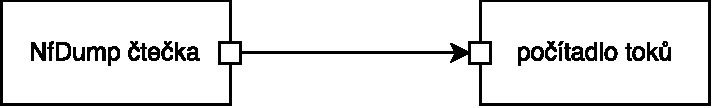
\includegraphics[width=0.5\textwidth]{fig/nemea-basic.pdf}
    \caption{Minimální příklad NEMEA systému obsahující pouze dva moduly.} \label{fig:nemea-schema}
  
\end{figure}

Z takovýchto základních bloků lze postavit i velmi komplexní systém jak je vidět na obrázku \ref{fig:nemea-example-2}, kde jsou data přijímána v reálném čase z IPFIX\cite{ipfix} kolektoru. Data jsou předzpracována, analyzována několika algoritmy a následně jsou nahlášeny detekované události. Každá z těchto úloh je jeden modul, který může být znovu použitý na několika různých místech.

\begin{figure}[h]
    \centering
    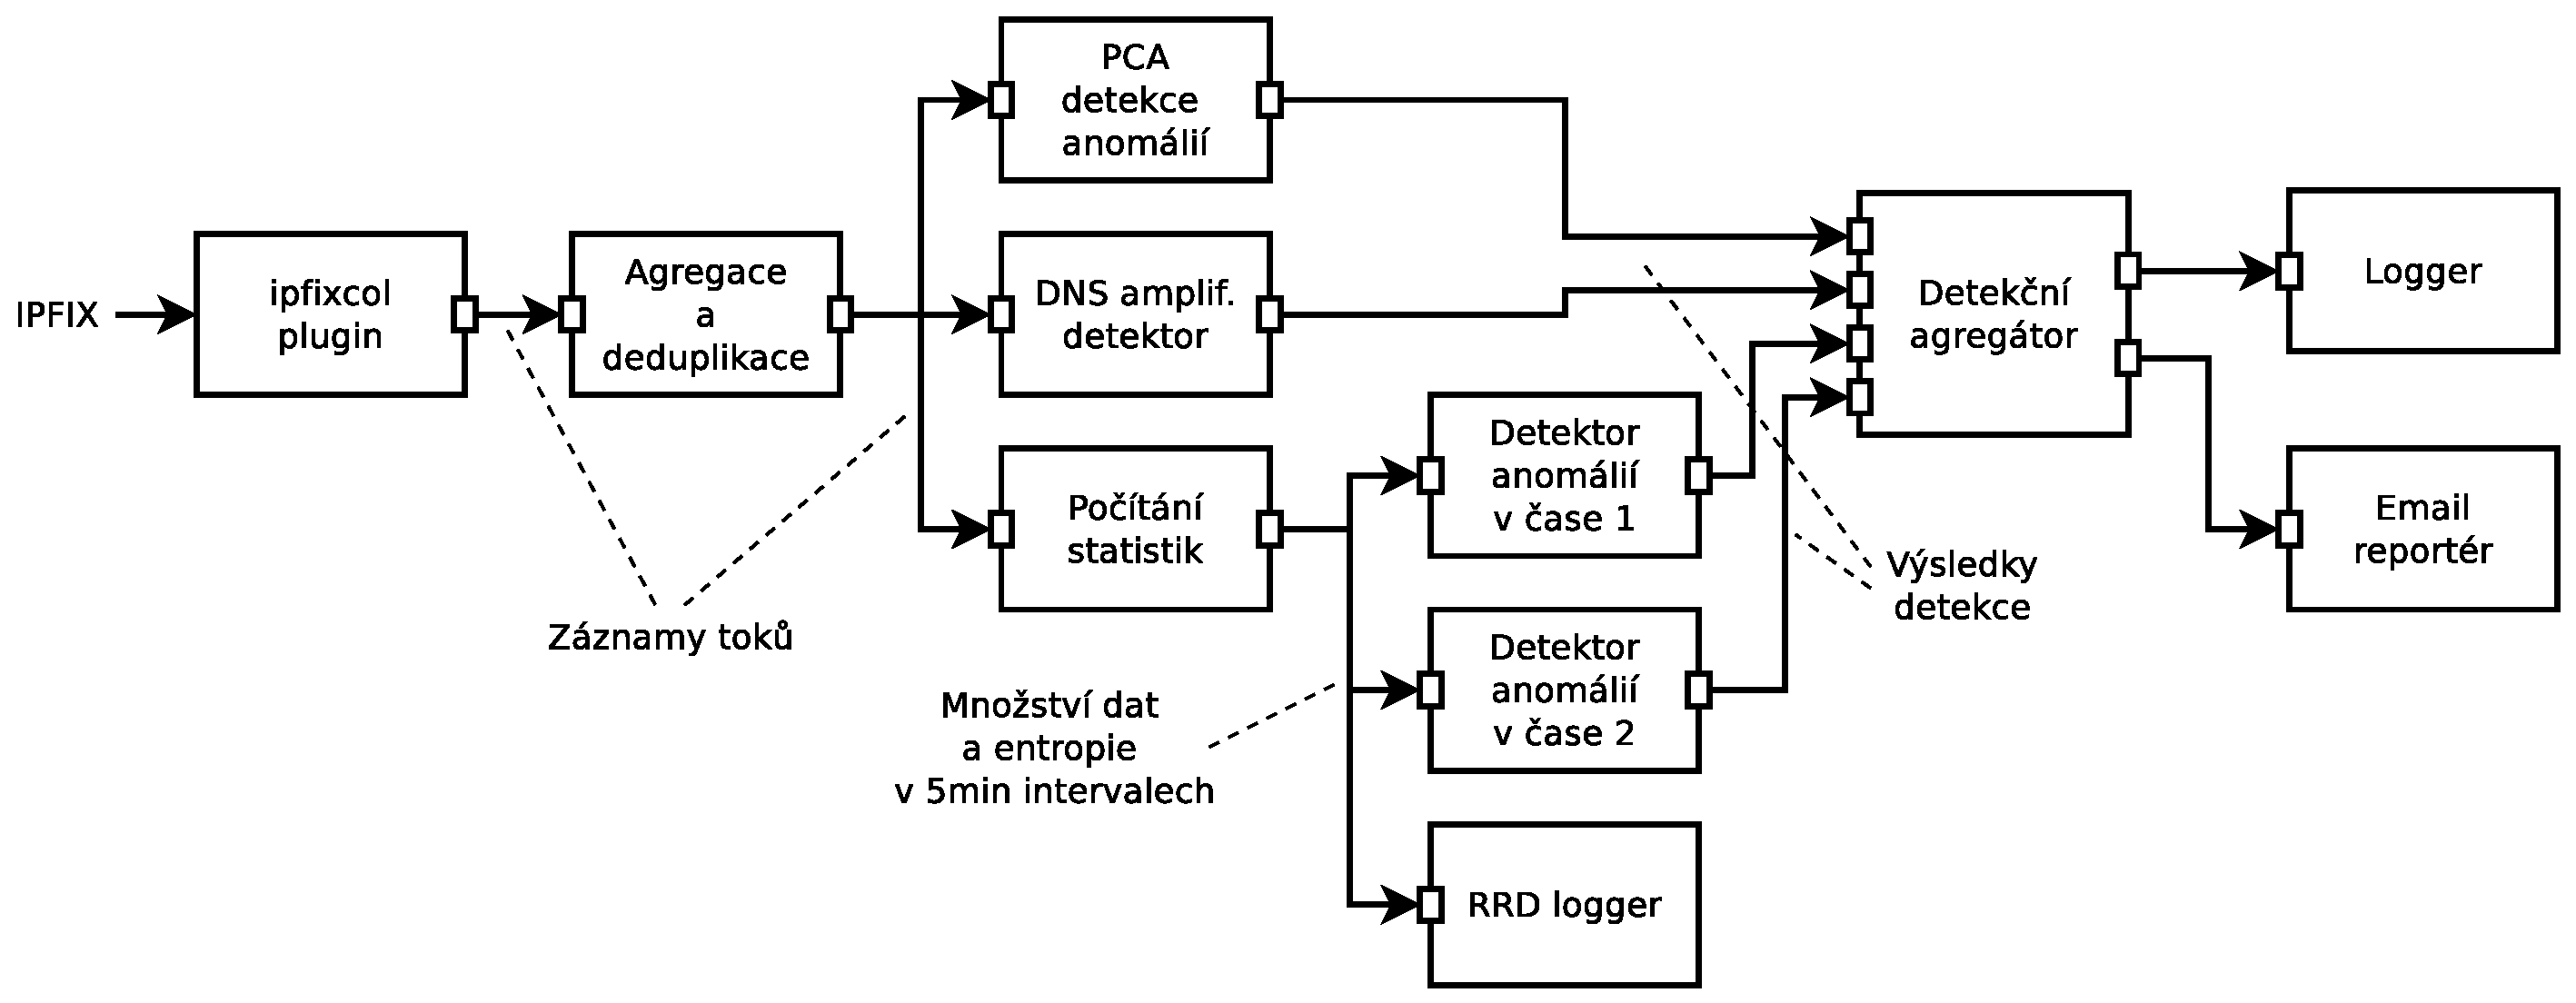
\includegraphics[width=1\textwidth]{fig/nemea-example-2-cz.eps}
    \caption{Příklad propojení modulů NEMEA systému, který shromažďuje síťová data, detekuje anomálie a útoky a následně události ukládá a reportuje.} \label{fig:nemea-example-2}
  
\end{figure}


%\subsection*{Hlavní komponenty}

\subsection{Modul}

Každý modul je samostatný program nezávislý na ostatních. To sice zvyšuje nároky na systém, ale dovoluje větší variabilitu při návrhu modulu. Ten je, díky tomuto návrhu, možno naprogramovat v libovolném jazyce, sledovat a řídit spotřebu zdrojů každého modulu zvlášť a zejména v případě nefungujícího modulu se celý systém NEMEA dokáže zotavit z chyby naprosto bez problémů. Modulární systém navíc dovoluje přidávat a odebírat jednotlivé moduly za běhu, což je v produkčním prostředí jedna ze základních vlastnostní kvalitního monitorovacího systému.

Při zapojení a startu nového modulu se modul periodicky snaží připojit na definované rozhraní. Pokusy o spojení jsou sledovány NEMEA Supervisorem, kterým lze spravovat všechny moduly v systému a pokud se modulu nepodaří po několika pokusech připojit na rozhraní, je modul ukončen.

\subsection{Rozhraní}

Všechny rozhraní jsou výhradně jednocestná a přenos dat je realizován formou jednotlivých záznamů. Všechny záznamy poslané přes jedno konkrétní rozhraní mají vždy stejný formát, nicméně mezi rozhraními se formát může lišit. 

Protokol pro dynamickou tvorbu formátu je nazván UniRec. Ten specifikuje nejen formát záznamu, ale také jak záznam vytvořit a jak zpracovat -- implementuje formát pro binární reprezentaci síťového záznamu.

Pro tvorbu rozhraní je vytvořena sdílená knihovna libtrap, která využívá Traffic Analysis Platform (zkráceně TRAP) pro komunikaci mezi různými rozhranímia tyto rozhraní využívají protokolu UniRec.

\section{IDEA}
\label{sec:idea}

Pro potřebu sdílení informací o síťových událostech mezi různými skupinami a zařízeními (např. honeypoty, analyzéry systémových zpráv, analyzéry provozu na síti, netflow sondy a další) existuje několik formátů záznamu pro takovéto události. Nicméně žádný z nich není natolik univerzální, aby byl vždy a všude použitelný a pokud se k takovému formátu blíží, tak není natolik detailní, aby pokryl všechny důležité informace.

IDEA, neboli Intrusion Detection Extensible Alert, je formát záznamu síťové události specifikovaný sdružením CESNET. IDEA si klade za cíl specifikovat takový formát záznamu, který je univerzální, přenositelný, ale zároveň dost konkrétní a snadno pochopitelný bez potřeby rozsáhlé dokumentace k jednotlivým polím.

Vzorový záznam generovaný systémem NEMEA je vyobrazený ve výpisu \ref{code:idea}. Jak je vidět, formát je specifikovaný jako JSON dokument, aby byl přehledný, čitelný v běžné podobě (narozdíl od binárních formátů), lehce přenositelný a efektivní (např. oproti XML\cite{xmlvsjson}).

%\vspace{5mm}
\begin{figure}[h]
\lstset{basicstyle=\small,style=JSON}
\begin{lstlisting}
{
    "Format" :      "IDEA0",
    "ID" :          "73e0b136-aeb8-4aae-bb80-9bfb4f258847",
    "Category" :    ["Availibility.DDoS"],
    "Description" : "DNS amplification",
    "EventTime" :   "2016-04-07T22:19:25Z",
    "CreateTime" :  "2016-04-07T22:34:52Z",
    "CeaseTime" :   "2016-04-07T22:34:38Z",
    "DetectTime" :  "2016-04-07T22:34:38Z"
    "PacketCount" : 393,
    "Source" : [{
        "IP4" : ["192.1.0.201"],
        "Proto" : ["udp","dns"],
        "OutPacketCount" : 393,
        "InPacketCount" : 767
    }],
    "Target" : [{
        "Proto" : ["udp","dns"],
        "IP4" : ["10.0.0.135"],
        "InPacketCount" : 393
    }],
    "Node" : [{
        "SW" : ["NEMEA","amplification_detection"],
        "Name" : "cz.cesnet.nemea.amplification_detection"
    }],
    "Type" : ["Flow","Statistical"],
}
\end{lstlisting}
\captionof{lstlisting}{Vzorový IDEA záznam ze systému NEMEA. Některé části byly vynechány nebo zkráceny a IP adresy změněny na lokální.}
\label{code:idea}
\end{figure}

\newpage

\section{Další monitorovací systémy}

Na trhu jsou v současné době různá dostupná řešení pro detekci a vizualizaci síťových bezpečnostních událostí, nicméně valná hromada z nich je komerční a hlavně vázaná na konkrétní hardware od daného výrobce. Klient tudíž většinou nekupuje software, ale hardware s přiloženým software.

Komerčně dostupný produkt je např. Flowmon\cite{flowmon:report} ADS\cite{flowmon:ads} od stejnojmenné společnosti. Flowmon je spin-off společností z projektu Liberouter ze sdružení CESNET. Jejich sondy a kolektory využívají technologie vytvořené ve sdružení CESNET jak z hlediska hardware, tak software. Dalším komerčním řešením je Cisco Secure IDS\cite{cisco:ids}, dříve známý jako Cisco NetRanger.

Open source projekty jako NEMEA jsou dostupné mnoho let, ale pouze několik z nich dosáhlo znatelnějšího rozšíření v komunitě síťových správců. Nejvýznamnějšími jsou systémy Snort\cite{snort}, VERMONT\cite{vermont} a framework Bro\cite{bro}. 

\subsection*{Snort}
Tento open-source projekt, od roku 2013 vlastněn firmou Cisco\cite{snort:cisco}, je možno konfigurovat ve 3 hlavních režimech\cite{snort:modes}: \uv{sniffer}, paket logger a jako (N)IDS. V režimu IDS Snort pracuje principiálně velmi podobně jako systém NEMEA. Zachytává síťový provoz, ukládá si důležité informace o něm a analyzuje jej. Ve výsledku ukládá záznamy o síťových událostech. Nicméně Snort není modulárním systémem a tudíž není tak flexibilní a není stavěný na vysokorychlostní rozsáhlé sítě jako systém NEMEA.

\subsection*{VERMONT}

VERMONT (Versatile Monitoring Toolkit) je modulární monitorovací systém obsahující IPFIX kolektor, exportér, analyzátor a další moduly a grafické prostředí pro vizuální analýzu dat. VERMONT byl vyvinut v rámci projektu HISTORY\cite{vermont:history} a evropským projektem DIADEM firewall\cite{vermont:diadem}. Svou architekturou je nejbližší systému NEMEA, protože je částečně modulární. Systém NEMEA je oproti tomu modulární od samotného jádra systému, což dovoluje vyšší flexibilitu při vývoji a menší závislost na použitých technologií.

\subsection*{Bro}
Dalším v komunitě rozšířeným řešením je framework Bro. Tento framework primárně určený pro síťovou analýzu není podobný systému NEMEA, ani předchozím systémům, protože je to spíše nástroj pro vytváření (N)IDS než-li ucelený systém. Bro se velmi blíží skriptovacímu jazyku (např. Perl) nebo unixovým nástrojům jako tcpdump nebo nfdump. Bro lze rozdělit na dvě vrstvy. První vrstvou je \uv{Bro Event engine}, který analyzuje síťový provoz a generuje neutrální síťové události v podobě \uv{byla vytvořena nějaká událost}. 

Tyto neurčité události jsou následně analyzovány druhou vrstvou -- \uv{Bro Policy skripty}. V této vrstvě je naimplementovaný zmiňovaný skriptovací jazyk. V současné době existuje mnoho naprogramovaných skriptů, které jsou připraveny k okamžitému použití, včetně pokročilé analýzy síťového provozu.

V ranných fázích vývoje se systém NEMEA velmi blížil frameworku Bro, s vývojem času se ale NEMEA stala uceleným systémem připraveným k okamžitému nasazení na měřící body.

\section{Shrnutí}

V této kapitole jsme prezentovali systém NEMEA a jeho architekturu. Popsali jsme jeho nejdůležitější části, zejména jak vypadá modul a jeho komunikační protokol. Dále jsme popsali formát záznamu síťové bezpečnostní události IDEA, který je opěrným bodem pro ukládání dat v systému NEMEA v rámci analýzy událostí koncovým uživatelem. V poslední sekci jsme porovnali systém NEMEA s dalšími veřejně dostupnými monitorovacími systémy.

%%%%%%%%%%%%%%%%%%%%%%%%%%%%
% Kapitola 3
% Technologie
%%%%%%%%%%%%%%%%%%%%%%%%%%%%

\chapter{Technologie}

Vizualiace síťových bezpečnostních událostí může být vytvořena několika postupy. Pokud máme IDS, který je dostupný pouze z jednoho stroje, nejčastěji zvolíme tvorbu desktopové aplikace, protože máme jistotu provozního prostředí jako je např. operační systém, dostupné balíčky a jejich verze, atd. V případě vzdálené správy IDS (častější případ) jsme nejčastěji odkázání na vzdálený přístup pomocí příkazové řádky. Tento přístup je bohužel velmi limitovaný a nelze jej využít pro vizualiaci. V současné době je pro vzdálenou správu nejvhodnější vytvořit webovou aplikaci, která je dostupná z Internetu a použitelná na většině dnes používaných zařízeních\footnote{Jedná se zejména o stolní počítače, notebooky, tablety a chytré mobilní telefony.}

Pro tvorbu moderních webové aplikace je na Internetu dostupná celá řada knihoven, frameworků a systémů. Nicméně první otázkou zůstává co taková moderní webová aplikace je?

Ustáleným pojmem pro moderní webovou aplikaci je z anglického single page application\cite{spa} zkratka \uv{SPA}.

Specifikem SPA je její vysoká interaktivita s uživatelem, vysoká dostupnost služby, kterou poskytuje a rozdělení na dva logické celky. Uživatelskou a serverovou část, často chybně nazývané frontend a backend aplikace. Více o architektuře aplikace v kapitole \ref{architektura}.

Většinu z těchto kvalit získává SPA díky způsobu jakým je doručována uživateli. SPA je při prvním načtení stránky v prohlížeči celá uložena v rámci vyrovnávací paměti prohlížeče a během celé doby použivání SPA není nutné stránku znova načítat. SPA můžeme chápat jako univerzálního klienta pro obsluhu dané aplikace. 

SPA je nejčastěji tvořena pomocí jazyka JavaScript. Ten umožňuje dynamickou změnu stránky bez nutnosti ji znova načítat a tím pádem uživatel nepřichází o dočasná data na stránce. Tento přístup navíc redukuje počet dotazů na server a snižuje tak jeho zátěž.

S přesunem logiky na uživatelskou část SPA jsou ale spojeny nemalé problémy. Zejména pak různorodá interpretace kódu. To se v posledních letech téměř eliminovalo díky moderním prohlížečům a jejich jádrům jako je např. WebKit pro Google Chrome nebo Gecko pro Firefox.

\section{Uživatelská část}

K vytvoření SPA a zejména uživatelské části existuje několik významných systémů. V této části si tyto technologie představíme a porovnáme mezi sebou. Nejdůležitější částí je JavaScriptová knihovna/framework, který bude nejčastěji interagovat s uživatelem. Další nedílnou součástí je knihovna pro HTML/CSS, která bude definovat vzhled aplikace.

\subsection{JavaScript MVC frameworky}

Bylo vybráno 5 JavaScript frameworků, které napomáhají k tvorbě SPA. Architektura MVC rozděluje aplikaci na tři celky, které mezi sebou navzájem komunikují. Více informací o MVC architektuře v kapitole \ref{architektura}.

Kritéria užšího výběru frameworků byla zejména následující:

\begin{itemize}  
\item open-source projekt s MIT nebo BSD licencí,
\item jednoduché použití,
\item relativně nenáročný na výpočetní výkon hostitelského stroje,
\item široká podpora mezi prohlížeči,
\item projekt má určitou historii a je udržován některou ze známých společností (udržitelnost vývoje).
\end{itemize}

\subsubsection*{React\cite{react}}
Framework React je vyvíjen pod hlavičkou společnosti Facebook. Původním cílem návrhářů Reactu bylo vyřešit problémy během vývoje komplexních uživatelských rozhraní s rychle měnícími se daty. Dalším cílem bylo vytvořit takový framework, který lze distribuovat v takovém měřítku jako je Facebook.

React je framework pro uživatelskou část SPA používající tradiční MVC architekturu. Taková architektura je nejvíce znatelná v případě použití obousměrného vázání dat (anglicky two-way data binding), více v sekci \ref{sec:mvc}.

React se zaměřuje zejména na tvorbu UI, z pohledu architektury pohledová část (view), a kvůli tomu se ostatním částem architektury nevěnuje tak detailně, jak by většinu času vývojář potřeboval. Velmi častým řešením je použít React na pohledovou část a na model a kontrolér použít jiný framework, např. AngularJS.

React pracuje s moderními přístupy k vývoji SPA a boří tak mnoho zažitých technik jak takovou PSA vyvíjet. Místo běžné manipulace s DOM elementy si React, případně vývojář, definuje vlastní DOM elementy, kterým přídává vlastnosti, váže na ně data a manipuluje s nimi bez větších výkonových ztrát. Toho docílil zejména použitím tzv. shadow DOM\cite{shadowdom}, který je ale novinkou na poli prohlížečů a je podporován pouze jádrem WebKit. 

%Pokud není shadow DOM dostupný, používá React standardní DOM, se kterým je sice vykreslování pomalejší, ale stále velmi rychlé. 

\begin{figure}[ht]
\lstset{basicstyle=\small,style=JSON}
\begin{lstlisting}
var HelloMessage = React.createClass({
    render: function() {
        return <div>Hello {this.props.name}</div>;
    }
});

ReactDOM.render(<HelloMessage name="John" />, mountNode);
\end{lstlisting}
\captionof{lstlisting}{\uv{Hello World} příklad v jazyku JSX, který do stránky vykreslí text \uv{Hello John}.}
\label{code:react}
\end{figure}

Pro názornou ukázku, jak framework React funguje, je ve výpise \ref{code:react} vytvořen jednoduchý \uv{Hello World} element v JSX\cite{jsx} syntaxi. Tento kód demonstruje pouze minimální možnosti frameworku, ale vypovídá o jednoduchosti použití Reactu.

\subsubsection*{Ember.js}

Ember.js je primárně zaměřen na tvorbu SPA. Toho dosahuje zejména používáním zažitých praktik v rámci komunity vývojářů, širokou funkcionalitou bez nutnosti instalace dalších doplňků a osvědčil se i vysokou stabilitou během celé doby vývoje. Ember je také vždy jedním z prvních frameworků, který implementuje novinky obsažené v nových jádrech webových prohlížečů jako jsou např. JavaScript Promises\cite{jspromises}, Web Components\cite{webcomponents} nebo ES6 syntaxe.

Ember se skládá celkem z pěti klíčových konceptů. Jejich názvy jsou ponechány anglicky pro větší názornost.

\begin{itemize}  
    \item {\bf Routes} -- každý stav aplikace je reprezentován unikátní cestou a této cestě náleží i odpovídající objekt, který manipuluje s danou cestou.
    \item {\bf Models} -- každá cesta má svůj korespondující model, který obsahuje data asociována s danou cestou a stavem aplikace. Model slouží zejména k manipulaci s daty.
    \item {\bf Templates} -- šablony jsou tvořeny v HTML s použitím šablonovacího jazyka HTMLBars\cite{htmlbars}.
    \item {\bf Components} -- komponenta je vlastní HTML značka definovaná programátorem aplikace. Její chování je implementováno pomocí JavaScriptu a její vzhled pomocí HTMLBars šablon. Komponenta se chová jako běžný DOM element.
    \item {\bf Services} -- servis je singleton objekt, který v sobě udržuje dlouhodobá data během používání aplikace klientem.
\end{itemize}

\subsubsection*{AngularJS}

AngularJS je jedním z nejdéle existujících frameworků pro tvorbu SPA. Je udržován společností Google a poskytuje ucelené prostředí k vývoji komplexních SPA. AngularJS poskytuje dvě metodiky návrhu architektury aplikace. MVC a MVVM (model-view-viewmodel)\cite{mvvm}.

MVVM je rozdílný zejména ve způsobu nakládání s daty v aplikaci. Viewmodel pouze reflektuje změny modelu v pohledu a naopak. Viewmodel lze chápat jako interpret dat získaných z modelu, které jsou požadovány v pohledu.

Vzhledem k rozsáhlosti frameworku se nevyhneme tvorbě aplikace, která prolíná oba typy architektury. AngularJS je ale zejména stavěn na základech MVC architektury.

AngularJS staví na několika základních cílech:

\begin{itemize}
    \item rozdělit manipulaci DOM od aplikační logiky,
    \item rozdělit klientskou a serverovou stranu aplikace,
    \item poskytnout strukturu pro vývoj SPA.
\end{itemize}

Manipulace s DOM je zajišťována v pohledové části architektury. Aplikační logika je v tomto případě oddělena a to dovoluje simultánní tvorbu na obou částích aplikace. To dovoluje strukturovat kód do uzavřených logických celků, které mohou být znovu použity v dalších částech aplikace.

Rozdělením klientské a serverové strany aplikace získává AngularJS celkovou kontrolu nad klientskou stranou a dokáže tak abstrahovat jednotlivé vrstvy aplikace. To dovoluje hlubokou integraci MVC architektury do klientské části.

Toto rozdělení dovoluje frameworku implementovat takové možnosti jako je např. vkládání závislostí nebo pohledově závislé kontroléry.

To vše spěje ke snížení zátěže serveru, na kterém je SPA uložena. Většina, ne-li všechna, aplikační logiky totiž probíhá na klientské straně a server pro svou práci vůbec nepotřebuje. Ten je potřeba až v momentě kdy chceme získat nebo uložit data pro dlouhodobé užití.

\subsubsection*{Backbone.js}

Framework Backbone.js se mírně odlišuje od předešlých a to svou architekturou, která není MVC, ale MVP (model-view-presenter). Presenter je v tomto modelu prostředníkem, který plní logickou funkci a spojuje pohled s modelem. Veškeré akce, které se provedou v pohledu (např. kliknutí na tlačítko) jsou delegovány presenteru. Ten je navíc oddělen od pohledu a komunikuje s ním pouze přes definované rozhraní.

Tento přístup je vhodný zejména pro testování a jasné oddělení jednotlivých částí (zvláště modelu od pohledu). Avšak MVP je náročnější na tvorbu kvůli tomu, že všechny datové vazby musí vytvořit sám programátor.

Výhodou Backbone.js je jeho velikost (celková velikost distribuce je méně než 8 kB) a nezávislost na dalších knihovnách (vyžaduje pouze jednu další knihovnu\footnote{Underscore.js, pokud chce programátor využít i složité funkce, musí navíc doplnit knihovnu jQuery.}).

Z předcházejících faktů lze vyvodit, že Backbone.js je vhodný zejména pro SPA menšího rozsahu, které jsou zaměřeny na velmi konkrétní úkol. To může v pozdějších fázích vývoje SPA znamenat problémy a kompromisy při vývoji další funkcionality aplikace.

\subsubsection*{Shrnutí}

Pro rychlý a stručný přehled byla vypracována tabulka shrnující klíčové vlastnosti každého porovnávaného frameworku.

\begin{table}[ht]
\centering
\caption{Porovnání klíčových vlastností JavaScript frameworků}
\label{tab:js}
\begin{tabular}{|l|l|l|l|l|}
\hline
    Název       & 
    Verze\tablefootnote{Aktuální verze v době psaní práce.}     & 
    Aktivní vývoj     & 
    Velikost\tablefootnote{Velikost minifikovaného produkčního kódu.}  & 
    Licence   \\ \hline
    React       & 15.0.1    & 3 roky (2013)     & 142 kB    & BSD       \\
    Ember.js    & 2.5.0     & 4 roky (2011)              & 450 kB    & MIT       \\
    Backbone.js & 1.3.3     & 5 let (2010)              & 7.5 kB    & MIT       \\
    AngularJS   & 1.5.3     & 5 let (2010)              & 152 kB    & MIT       \\
\hline
\end{tabular}
\end{table}

\newpage

\subsection{HTML/CSS frameworky}

Důležitým aspektem SPA je také její vzhled, nebo spíše UX (user-experience)\cite{ux:iso}. UX je zejména vnímání a reakce osoby, které plyne z používání nebo předpokládaného užití/chování výrobku, systému nebo služby. Důraz se musí klást zejména na předpokládáné chování systému, tím pádem může uživatel procházet plynule aplikací, aniž by musel odhadovat chování té části aplikace, ve které se právě nachází.

Toho lze dosáhnout zejména uceleností vzhledu a chování jednotlivých komponent SPA. Pro tento účel existují tzv. HTML/CSS knihovny. Na Internetu je jich velké množství a výběr jsem zúžil pouze na 3 knihovny, které jsou známé; mají širokou škálu komponent, které lze v SPA využít a jsou open-source.

Poslední podmínkou jsou zdrojové kódy CSS v jednom z CSS preprocesorů\cite{css:preproc} -- LESS\footnote{\url{http://lesscss.org}} nebo SASS\footnote{\url{http://sass-lang.com}}, aby v aplikaci byla zaručena konzistence proměnných (např. barvy, velikost, odsazení).

\subsubsection*{Bootstrap}

Bootstrap je nejpopulárnějším frameworkem pro tvorbu vzhledu SPA. Obsahuje HTML a CSS komponenty pro ucelenou typografii, formuláře, tlačítka, navigaci a další. Bootstrap také nabízí komponenty, které jsou částečně nebo zcela napsány v JavaScriptu.

Bootstrap je udržován zejména společností Twitter, kde také vznikl na popud tvorby interních firemních aplikací s uceleným vzhledem a také UX, aby se ušetřily náklady na údržbu takovýchto aplikací.

Díky Bootstrapu se velmi rychle ujal trend responzivního designu a mobile-first přístupu. Navíc disponuje velkou komunitou vývojářů a časté problémy jsou tak mnohokrát vyřešeny.

\subsubsection*{Foundation}

Foundation je velmi podobný framework jako Bootstrap, také nabízí HTML a CSS komponenty pro různé části SPA včetně JavaScript komponent. Nemá sice za sebou takovou společnost jakou je Twitter, ale je neméně kvalitní a udržovaný.

Hlavním rozdílem oproti Bootstrapu je jeho upravitelnost. Foundation dává větší prostor pro úpravu jednotlivých komponent. 

Navíc disponuje styly, které jsou automaticky aplikované na dané HTML elementy -- vývojář nepotřebuje přidávat množství tříd ke každému elementu. To však nemusí každému vyhovovat a mohou nastat neobvyklé konflikty stylů během vývoje.

\subsubsection*{Angular Material}

Angular Material není běžným CSS frameworkem, nýbrž je velmi úzce spjat s JavaScript frameworkem AngularJS a využívá jeho mnoha možností jako jsou např. vlastní HTML elementy (direktivy).

Framework také obsahuje mnoho HTML a CSS komponent, ale ty jsou vždy velmi úzce spjaty s AngularJS funkcionalitou jako je např. two-way data binding a již zmíněné direktivy. 

Společnost Google disponuje vizuálním jazykem pro všechny své produkty nazvaný Material Design\footnote{\url{https://www.google.com/design/spec/material-design/introduction.html}}. Ten je založený na tzv. \uv{kartičkách}, které lze skládat na sebe, řadit, organizovat a upravovat.

Jak již název frameworku napovídá je tento vizuální jazyk použit skrz všechny dostupné komponenty.

Z technického hlediska je Angular Material nejpokročilejším frameworkem. Pro mřížkový systém\footnote{angl. grid system} používá flexbox, který je dostupný pouze v nejnovější specifikaci CSS 3 a moderních webových prohlížečích. To může způsobit vážné problémy, pokud je SPA cílena na široké publikum.


\section{Serverová část}

\subsection{REST API}

\subsubsection*{Python Flask}
\subsubsection*{PHP}
\subsubsection*{C++ a Mongoose}
\subsubsection*{NodeJS}





\section{Vybrané technologie}
\subsection{Uživatelská část}

\subsection{Serverová část}

%\section{Zvolené technologie}

\chapter{Architektura aplikace}
\label{architektura}

\begin{figure}[h]
    \centering
    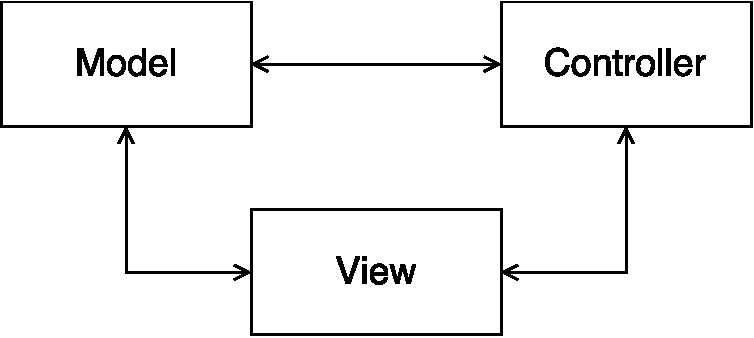
\includegraphics[width=0.5\textwidth]{fig/mvc.pdf}
    \caption{MVC architektura} \label{fig:mvc}
  
\end{figure}

\section{MVC}
\label{sec:mvc}


\section{Případy užití}
\section{REST API}
\section{Databáze událostí}
\section{GUI}

\chapter{Implementace}
\section{Backend}
\section{Frontend}
\section{Zabezpečení}
\section{Distribuce}

\chapter{Dosažené výsledky}
%\section{Názory uživatelů}
%\section{Nasazení v praxi}

\chapter{Závěr}
Závěrečná kapitola obsahuje zhodnocení dosažených výsledků se zvlášť vyznačeným vlastním přínosem studenta. Povinně se zde objeví i zhodnocení z pohledu dalšího vývoje projektu, student uvede náměty vycházející ze zkušeností s řešeným projektem a uvede rovněž návaznosti na právě dokončené projekty.

%=========================================================================
